\documentclass[crop,tikz]{standalone} 
\usepackage{tikz, amsmath, amssymb, graphicx} 

\DeclareMathAlphabet\mathbfcal{OMS}{cmsy}{b}{n}

\newcommand{\Mt}{\mathbfcal{M}}
\newcommand{\Yt}{\mathbfcal{Y}}
\newcommand{\Ft}{\mathbfcal{F}}

\usetikzlibrary{positioning, shapes.geometric} 

\begin{document} 

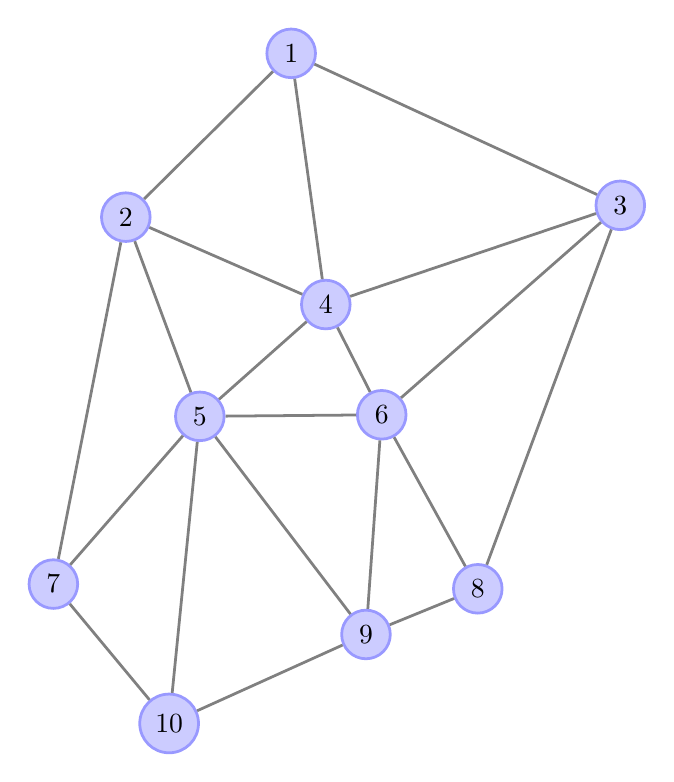
\begin{tikzpicture} 


\tikzstyle{node_style} = [circle,draw=blue!40!,fill=blue!20!, line width=1]
\tikzstyle{edge_style} = [draw=gray, line width=1]

\node[node_style] (v0) at (4.17, 4.19) {6};
\node[node_style] (v1) at (7.20, 6.85) {3};
\node[node_style] (v2) at (0.00, 2.04) {7};
\node[node_style] (v3) at (3.02, 8.78) {1};
\node[node_style] (v4) at (1.47, 0.27) {10};
\node[node_style] (v5) at (0.92, 6.70) {2};
\node[node_style] (v6) at (1.86, 4.17) {5};
\node[node_style] (v7) at (3.46, 5.59) {4};
\node[node_style] (v8) at (3.97, 1.40) {9};
\node[node_style] (v9) at (5.39, 1.98) {8};

\draw[edge_style]  (v0) edge (v9);
\draw[edge_style]  (v0) edge (v8);
\draw[edge_style]  (v0) edge (v7);
\draw[edge_style]  (v0) edge (v6);
\draw[edge_style]  (v0) edge (v1);
\draw[edge_style]  (v1) edge (v9);
\draw[edge_style]  (v1) edge (v7);
\draw[edge_style]  (v1) edge (v3);
\draw[edge_style]  (v3) edge (v7);
\draw[edge_style]  (v3) edge (v5);
\draw[edge_style]  (v6) edge (v7);
\draw[edge_style]  (v5) edge (v6);
\draw[edge_style]  (v6) edge (v8);
\draw[edge_style]  (v2) edge (v5);
\draw[edge_style]  (v2) edge (v6);
\draw[edge_style]  (v2) edge (v4);
\draw[edge_style]  (v4) edge (v6);
\draw[edge_style]  (v4) edge (v8);
\draw[edge_style]  (v8) edge (v9);
\draw[edge_style]  (v7) edge (v5);



 
% \draw [green, dashed] (1, -2.7) rectangle (2.05, 0.3);

% \node [below, opacity=0, text opacity=1] at (2.45, -1) {$\otimes$};

% \draw [blue, dashed] (2.9, -2.7) rectangle (6.5, 0.3);
% \node[inner sep=0pt] (subjects) at (6.2, -0.2) {};

% \node [below, opacity=0, text opacity=1] at (6.9, -1) {$\otimes$};

% \draw [orange, dashed] (7.4, -2.7) rectangle (10.5, 0.3);
% \node[inner sep=0pt] (stimuli) at (10.3, -0.2) {\includegraphics[width=.22\textwidth]{fMRI_Stimuli_Diagram.pdf}};




\end{tikzpicture}
\end{document} 
